\chapter{Multiplicité, entropie et équilibre sous contraintes}

\lectureoverview{Une distribution de probabilité devient un objet thermodynamique dès lors que ses états sont associés à des énergies. Nous relions d’abord l’augmentation de l’entropie à l’équilibration et utilisons \(dE=T\,dS\) pour déduire le sens du flux thermique. Nous remplaçons ensuite un système par un grand ensemble de répliques, comptons les configurations associées à chaque ensemble de nombres d’occupation et montrons que le logarithme de cette multiplicité vaut l’entropie multipliée par \(N\). L’équilibre est donc un problème de maximisation de l’entropie sous contraintes. Les multiplicateurs de Lagrange fournissent la méthode nécessaire pour le résoudre.}

\section{Les trois grandeurs fondamentales}

Soit \(i\) un indice des états discrets accessibles au système. Pour l’instant, le caractère discret est utile, car il nous permet de compter les états sans introduire de mesures dans l’espace des phases. Si la probabilité de l’état \(i\) est \(P_i\), alors
\begin{equation}
 \sum_i P_i=1.
 \label{eq:sm3-normalization}
\end{equation}
Si l’énergie de cet état est \(E_i\), l’énergie moyenne vaut
\begin{equation}
 \overline E=\sum_iP_iE_i.
 \label{eq:sm3-mean-energy}
\end{equation}
Le mot \emph{moyenne} est important. Le système n’a pas nécessairement la valeur \(\overline E\) dans un état microscopique donné ; il s’agit de la moyenne pondérée par les probabilités sur les valeurs possibles.

\begin{classroomqa}
\classquestion{Y a-t-il ici une distinction utile entre probabilité et statistique ?}
\lecturerresponse{La probabilité fournit un modèle des résultats possibles, tandis que la statistique part généralement de données observées et cherche à déterminer ce qu’on peut en déduire. Le calcul présent fait appel à des distributions de probabilité, même si les mêmes moyennes apparaissent naturellement dans les données statistiques. Dans l’échange informel en classe, ces termes sont employés sans trop de rigueur, car cette distinction n’a pas d’incidence sur la physique qui suit.
\lecturetimestamp{00:01:39--00:02:21}}
\end{classroomqa}

L’entropie de la distribution est
\begin{equation}
 S[P]=-\sum_iP_i\log P_i.
 \label{eq:sm3-entropy}
\end{equation}
Cette expression est non négative. Toute probabilité non nulle vérifie \(0<P_i\leq1\), donc \(\log P_i\leq0\), et la valeur limite conventionnelle \(P_i\log P_i\to0\) s’applique lorsque \(P_i\to0\).

\begin{figure}[t]
\centering
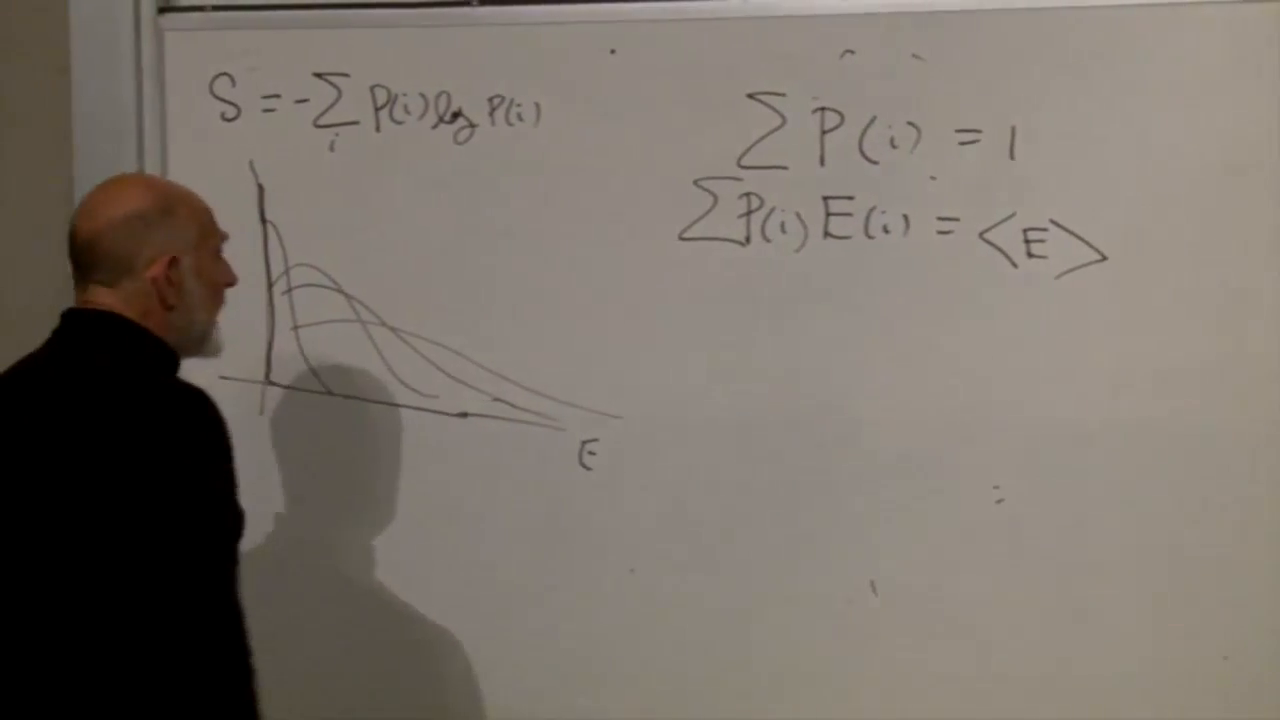
\includegraphics[width=0.88\textwidth]{lecture_03_figure_02.png}
\caption{Le tableau d’ouverture rassemble les formules de l’entropie, de la normalisation et de l’énergie moyenne, ainsi qu’une famille qualitative de distributions d’équilibre.}
\lectureframe{00:06:44}
\end{figure}

\section{L’équilibre comme famille de distributions}

Le cours précédent nous a laissé une famille de distributions d’équilibre à un paramètre. On peut paramétrer cette famille par la température, mais, pour l’instant, il est plus utile de la paramétrer par l’énergie moyenne \(\overline E\). À l’énergie minimale possible, la distribution est concentrée sur un état fondamental :
\[
 P_i=\delta_{i0}.
\]
L’état est alors connu sans incertitude, et \(S=0\). À mesure que la distribution d’équilibre s’étend à davantage de niveaux d’énergie, son énergie moyenne et son entropie augmentent toutes deux.

Il s’agit d’une propriété de la famille thermique, et non de toute distribution que l’on pourrait imaginer. Une famille arbitraire pourrait se déplacer vers des énergies plus élevées tout en se resserrant. Les distributions d’équilibre que nous allons déduire ne se comportent pas ainsi dans le régime usuel de température positive. Le long de cette famille,
\begin{equation}
 \frac{dS}{d\overline E}>0.
 \label{eq:sm3-positive-temperature-branch}
\end{equation}
Les systèmes dont le spectre est borné peuvent aussi présenter des branches où cette dérivée est négative. Ces régimes de température négative existent bel et bien, mais nous les laissons de côté dans le présent raisonnement.

L’équilibre thermique ne signifie pas que les mouvements microscopiques cessent. Les molécules continuent de se déplacer, d’entrer en collision et d’échanger de l’énergie. C’est la description macroscopique qui devient stationnaire : la distribution ne présente plus de dérive nette, et les différentes parties du système ne sont plus parcourues par un flux net d’énergie.

\section{Les lois de la thermodynamique dans le langage statistique}

Le premier principe exprime la conservation de l’énergie. Le deuxième principe stipule que l’entropie thermodynamique d’un système macroscopique isolé ne diminue pas :
\begin{equation}
 \Delta S_{\mathrm{tot}}\geq0.
 \label{eq:sm3-second-law}
\end{equation}
Une égalité correspond à l’équilibre ou à une transformation idéale réversible ; une relaxation spontanée entraîne généralement une augmentation stricte.

Dans la description probabiliste, la relaxation tend à répartir le poids entre les possibilités macroscopiques que nous distinguons encore. Il faut assortir cette affirmation de la réserve soulignée pendant le cours : nous effectuons un \emph{regroupement grossier}. L’évolution hamiltonienne exacte conserve l’entropie fine dans l’espace des phases. L’entropie macroscopique augmente parce que nous cessons de suivre les corrélations et les détails microscopiques. La perte de ces informations élargit la description réduite. Un resserrement spontané signifierait au contraire que nous avons acquis des informations microscopiques sans effectuer de mesure.

Le principe zéro affirme que les systèmes peuvent atteindre l’équilibre thermique et que cette relation d’équilibre est transitive. Si \(A\) est en équilibre avec \(B\), et \(B\) avec \(C\), alors \(A\) est en équilibre avec \(C\). La température est la grandeur qui rend cette transitivité manifeste :
\[
 T_A=T_B,\qquad T_B=T_C
 \quad\Longrightarrow\quad
 T_A=T_C.
\]
Hors équilibre, l’énergie passe du sous-système dont la température est la plus élevée vers celui dont la température est la plus basse. À températures égales, le flux net cesse. Nous allons maintenant déduire cette affirmation opérationnelle de la définition de la température par l’entropie.

\section{Pourquoi l’énergie passe du chaud vers le froid}

Considérons deux sous-systèmes faiblement couplés, \(A\) et \(B\). Chacun est en équilibre interne, mais leurs températures diffèrent. Choisissons les indices de sorte que
\begin{equation}
 T_B>T_A>0.
 \label{eq:sm3-temperature-order}
\end{equation}
Lors d’un petit échange, la conservation de l’énergie totale donne
\begin{equation}
 dE_A+dE_B=0.
 \label{eq:sm3-energy-conservation}
\end{equation}
Le deuxième principe donne
\begin{equation}
 dS_A+dS_B\geq0.
 \label{eq:sm3-entropy-change}
\end{equation}
Pour chaque sous-système en équilibre interne, la température est définie par
\begin{equation}
 dE_X=T_X\,dS_X,
 \qquad X=A,B.
 \label{eq:sm3-temperature-differential}
\end{equation}
En substituant dans \eqref{eq:sm3-energy-conservation}, on obtient
\begin{equation}
 T_A\,dS_A+T_B\,dS_B=0,
\end{equation}
d’où
\begin{equation}
 dS_B=-\frac{T_A}{T_B}\,dS_A.
 \label{eq:sm3-dsb}
\end{equation}
En reportant ce résultat dans \eqref{eq:sm3-entropy-change},
\begin{align}
 dS_{\mathrm{tot}}
 &=dS_A-\frac{T_A}{T_B}dS_A\\
 &=\frac{T_B-T_A}{T_B}\,dS_A\geq0.
 \label{eq:sm3-flow-entropy}
\end{align}
Comme \(T_B-T_A>0\) et \(T_B>0\), un échange spontané exige
\[
 dS_A>0.
\]
L’équation \eqref{eq:sm3-temperature-differential} donne alors
\begin{equation}
 dE_A=T_A\,dS_A>0,
 \qquad
 dE_B=-dE_A<0.
 \label{eq:sm3-hot-to-cold}
\end{equation}
L’énergie est passée de \(B\), le sous-système le plus chaud, à \(A\), le plus froid. Ici, la chaleur désigne simplement l’énergie en transit. Le flux se poursuit jusqu’à ce que \(T_A=T_B\), lorsque la variation d’entropie au premier ordre ne favorise plus aucune direction.

On peut présenter le même résultat en une seule ligne :
\begin{equation}
 dS_{\mathrm{tot}}
 =dE_A\left(\frac{1}{T_A}-\frac{1}{T_B}\right)\geq0.
 \label{eq:sm3-compact-flow}
\end{equation}
Le signe de la différence des inverses des températures détermine le signe de \(dE_A\). Cette forme compacte s’accordera naturellement plus tard avec l’ensemble canonique.

\begin{classroomqa}
\audiencequestion{Ce raisonnement suppose-t-il que \(A\) et \(B\) sont déjà chacun en équilibre interne ?}
\lecturerresponse{Oui. Attribuer une seule valeur de \(T_A\) ou de \(T_B\) suppose cet équilibre. Si un sous-système n’est pas en équilibre interne, on le divise en régions plus petites et on applique localement le raisonnement partout où l’on peut définir une température. La relaxation globale résulte alors des échanges entre ces régions.
\lecturetimestamp{00:24:38--00:25:22}}
\end{classroomqa}

\section{Qu’entend-on par état ?}

Avant de chercher les probabilités d’équilibre, nous devons savoir ce que désigne l’indice \(i\). Un état microscopique est la description la plus complète du système que permettent les lois physiques sous-jacentes. En mécanique classique, on se représente les positions et les moments de toutes les particules. En mécanique quantique, un état est plutôt un état quantique complet ; le principe d’incertitude interdit de spécifier simultanément avec une précision arbitraire toutes les positions et tous les moments classiques.

Pour un système quantique dans une boîte finie, le dénombrement pertinent des états peut être discret. La mécanique statistique classique émerge dans une limite appropriée, où les sommes sur des états quantiques très rapprochés deviennent des intégrales dans l’espace des phases. Cette limite introduit aussi la cellule d’espace des phases nécessaire pour rendre l’entropie continue sans dimension ; elle ne s’obtient pas en remplaçant simplement un signe de sommation par un signe intégral.

\begin{classroomqa}
\audiencequestion{Pour un gaz, faut-il se représenter un état comme les positions et les moments de chaque molécule ?}
\lecturerresponse{C’est bien la représentation classique. Plus généralement, un état désigne tout ce qui pourrait en principe être connu du système, dans les limites imposées par les lois physiques. La mécanique quantique modifie la forme de cette description maximale et rend discret le dénombrement dans un volume fini. Retrouver l’intégrale classique à partir de la somme quantique exige une véritable démarche de passage à la limite ; ce n’est pas une substitution en une ligne.
\lecturetimestamp{00:25:31--00:27:38}}
\end{classroomqa}

\section{Un bain thermique constitué de répliques}

La question difficile se pose désormais inévitablement : une fois l’équilibre établi, qu’est-ce qui détermine \(P_i\) ?

Mettons le sous-système en contact avec un bain thermique de très grande taille. L’énergie peut passer dans les deux sens, mais le bain possède tellement de degrés de liberté qu’un petit transfert d’énergie modifie à peine sa température. Un bain particulièrement commode est constitué de nombreuses répliques du sous-système lui-même, faiblement couplées entre elles. Une réplique est le système étudié ; les autres constituent son environnement.

Cette construction correspond souvent à un véritable système macroscopique. Divisons un grand corps presque homogène en cellules semblables. Chaque cellule est un sous-système, et les autres cellules forment son bain. Notons \(N\) le nombre total de répliques. La démonstration en classe utilise neuf répliques et trois étiquettes d’état colorées, mais le dénombrement ne dépend pas de ces nombres particuliers.

Soit \(n_i\) le nombre de répliques dans l’état \(i\). Ce sont les \emph{nombres d’occupation}. Il peut exister une infinité de niveaux d’énergie, mais, à énergie totale finie, l’occupation de la plupart des niveaux très élevés est négligeable ou nulle.

La première contrainte porte simplement sur le nombre de répliques :
\begin{equation}
 \sum_i n_i=N.
 \label{eq:sm3-number-constraint}
\end{equation}
La seconde porte sur l’énergie totale :
\begin{equation}
 \sum_i n_iE_i=N\overline E.
 \label{eq:sm3-total-energy-constraint}
\end{equation}
Le membre de droite est une grandeur extensive. Si l’on double le nombre de répliques tout en maintenant leur état statistique, l’énergie totale double, tandis que l’énergie moyenne par réplique reste égale à \(\overline E\).

\begin{classroomqa}
\audiencequestion{La construction avec des répliques doit-elle aussi satisfaire une contrainte sur l’énergie ?}
\lecturerresponse{Oui. La somme des nombres d’occupation doit être égale à \(N\), et leur somme pondérée par l’énergie doit être égale à l’énergie totale fixée \(N\overline E\). Ce sont précisément les deux contraintes qui limiteront ensuite la maximisation de l’entropie.
\lecturetimestamp{00:37:12--00:39:54}}
\end{classroomqa}

La probabilité qu’une réplique choisie au hasard soit dans l’état \(i\) est sa fréquence relative :
\begin{equation}
 P_i=\frac{n_i}{N},
 \qquad
 n_i=NP_i.
 \label{eq:sm3-frequency-probability}
\end{equation}

\begin{figure}[t]
\centering
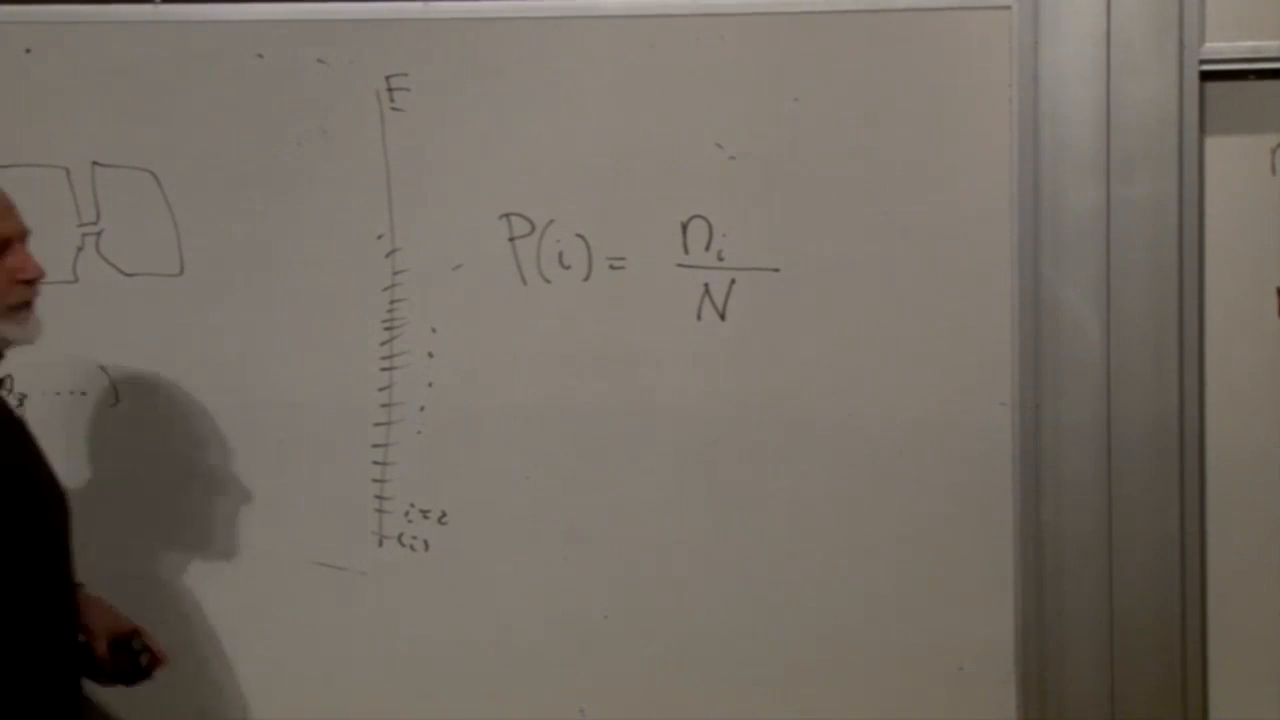
\includegraphics[width=0.82\textwidth]{lecture_03_figure_03.png}
\caption{Le schéma des niveaux d’énergie et l’identification de la probabilité à la fraction d’occupation \(P_i=n_i/N\).}
\lectureframe{00:41:40}
\end{figure}

\begin{classroomqa}
\audiencequestion{La notation \(N(i)\) au tableau est-elle censée différer de \(n_i\) ?}
\lecturerresponse{Non. Les deux désignent le nombre d’occupation de l’état \(i\). Nous utilisons systématiquement \(n_i\) et réservons la lettre majuscule \(N\) au nombre total de répliques.
\lecturetimestamp{00:41:28--00:41:33}}
\end{classroomqa}

En divisant \eqref{eq:sm3-number-constraint} et \eqref{eq:sm3-total-energy-constraint} par \(N\), on retrouve les contraintes sur les probabilités :
\begin{equation}
 \sum_iP_i=1,
 \qquad
 \sum_iP_iE_i=\overline E.
 \label{eq:sm3-probability-constraints}
\end{equation}
L’interprétation des fréquences dans l’ensemble a donc redonné les équations par lesquelles nous avons commencé.

\section{Multiplicité d’une configuration d’occupation}

Fixons un ensemble de nombres d’occupation \(\{n_i\}\). Combien d’affectations des \(N\) répliques discernables aux états réalisent exactement cet ensemble ? La réponse est le coefficient multinomial
\begin{equation}
 C(\{n_i\})=\frac{N!}{\prod_i n_i!}.
 \label{eq:sm3-multiplicity}
\end{equation}
Pour comprendre le dénominateur, commençons par ranger les \(N\) répliques étiquetées de \(N!\) façons. Permuter les \(n_i\) répliques qui occupent le même état ne produit pas une nouvelle affectation des occupations ; on divise donc par \(n_i!\) pour chaque état.

\begin{figure}[t]
\centering
\includegraphics[width=0.88\textwidth]{lecture_03_figure_04.png}
\caption{La multiplicité multinomiale
\(C=N!/\prod_i n_i!\) inscrite au tableau.}
\lectureframe{00:46:55}
\end{figure}

Les niveaux inoccupés ne posent aucun problème, car \(0!=1\). Si toutes les répliques occupent un même état, alors
\[
 C=\frac{N!}{N!}=1,
\]
comme prévu. Si trois répliques occupent trois états spécifiés distincts, alors
\[
 C=\frac{3!}{1!\,1!\,1!}=6.
\]
Avec deux répliques occupant deux états spécifiés, la formule donne deux affectations : on échange l’état occupé par chacune des répliques étiquetées.

\begin{classroomqa}
\audiencequestion{Plusieurs ensembles de nombres d’occupation peuvent-ils satisfaire les deux contraintes ?}
\lecturerresponse{En général, oui, il en existe beaucoup. L’équation \eqref{eq:sm3-multiplicity} compte d’abord les arrangements correspondant à un ensemble fixé \(\{n_i\}\), sans décider encore s’il satisfait les contraintes. À l’étape suivante, on compare tous les ensembles compatibles avec les contraintes pour déterminer lequel a la plus grande multiplicité.
\lecturetimestamp{00:48:07--00:48:43}}
\end{classroomqa}

L’hypothèse statistique consiste à traiter de façon symétrique les affectations microscopiques compatibles avec le système isolé. Une configuration macroscopique d’occupation réalisée par un plus grand nombre d’affectations est donc plus probable. Pour un grand \(N\), la distribution des fractions \(n_i/N\) présente un pic très marqué. Les fractions d’équilibre sont les valeurs qui maximisent \(C\) sous les contraintes \eqref{eq:sm3-number-constraint} et \eqref{eq:sm3-total-energy-constraint}.

\section{L’approximation de Stirling}

Les factorielles deviennent énormes bien avant que \(N\) n’atteigne une valeur macroscopique ; nous travaillons donc avec leurs logarithmes. Partons de
\begin{equation}
 \log N!=\sum_{x=1}^{N}\log x.
 \label{eq:sm3-log-factorial-sum}
\end{equation}
Pour un grand \(N\), la somme est approchée par l’aire sous \(\log x\) :
\begin{align}
 \log N!
 &\simeq\int_1^N\log x\,dx\\
 &=\left[x\log x-x\right]_1^N\\
 &=N\log N-N+1.
 \label{eq:sm3-stirling-integral}
\end{align}
La primitive se déduit immédiatement de
\[
 \frac{d}{dx}(x\log x-x)=\log x.
\]
Au premier ordre extensif, on peut négliger la constante additive :
\begin{equation}
 \log N!\simeq N\log N-N.
 \label{eq:sm3-stirling-log}
\end{equation}
En prenant l’exponentielle, on obtient la forme simplifiée utilisée dans le cours,
\begin{equation}
 N!\simeq N^N e^{-N}.
 \label{eq:sm3-stirling-simple}
\end{equation}

\begin{figure}[t]
\centering
\includegraphics[width=0.88\textwidth]{lecture_03_figure_05.png}
\caption{L’approximation de Stirling au premier ordre et sa dérivation, qui remplace la somme de \(\log x\) par une intégrale.}
\lectureframe{01:03:45}
\end{figure}

\begin{classroomqa}
\audiencequestion{L’évaluation de \(x\log x-x\) à la borne inférieure laisse-t-elle un terme supplémentaire \(+1\) ?}
\lecturerresponse{Oui. L’équation \eqref{eq:sm3-stirling-integral} contient cette constante. Elle est négligeable devant les termes proportionnels à \(N\) lorsque \(N\to\infty\), ce qui explique son omission dans la formule au premier ordre. La somme doit commencer à \(x=1\) ; \(\log0\) n’est pas défini.
\lecturetimestamp{01:04:12--01:04:35}}
\end{classroomqa}

\begin{classroomqa}
\audiencequestion{Un facteur proportionnel à \(\sqrt{N}\) manque-t-il aussi ?}
\lecturerresponse{Oui. La formule asymptotique plus précise est
\[
 N!\sim\sqrt{2\pi N}\left(\frac{N}{e}\right)^N.
\]
Son logarithme n’apporte qu’une contribution de \(\tfrac12\log(2\pi N)\), sous-extensive
par rapport à \(N\log N-N\). Elle importe pour calculer avec précision les
probabilités à \(N\) fini, mais pas pour le calcul de l’entropie au premier ordre d’un système macroscopique.
\lecturetimestamp{01:04:35--01:05:40}}
\end{classroomqa}

Il faut également appliquer avec précaution l’approximation de Stirling au dénominateur de \eqref{eq:sm3-multiplicity}. À la limite thermodynamique, les états dont les probabilités limites sont non nulles vérifient \(n_i=NP_i\) ; leurs occupations croissent donc avec \(N\). On peut traiter les états dont l’occupation est très faible ou nulle au moyen d’une coupure en énergie finie, puis rétablir la limite. Les termes sous-dominants omis ne modifient pas l’entropie extensive au premier ordre.

\section{Le logarithme de la multiplicité est l’entropie}

Appliquons \eqref{eq:sm3-stirling-simple} au numérateur et à tous les facteurs du dénominateur correspondant à des occupations macroscopiques :
\begin{equation}
 C\simeq
 \frac{N^Ne^{-N}}
 {\prod_i n_i^{\,n_i}e^{-n_i}}.
 \label{eq:sm3-c-stirling}
\end{equation}
Puisque \(\sum_i n_i=N\), les facteurs exponentiels dominants se simplifient :
\begin{equation}
 C\simeq\frac{N^N}{\prod_i n_i^{\,n_i}}.
 \label{eq:sm3-c-leading}
\end{equation}
Il est plus facile de maximiser un logarithme qu’un produit, et le logarithme étant une fonction croissante, les deux maxima correspondent à la même configuration d’occupation :
\begin{equation}
 \log C=N\log N-\sum_i n_i\log n_i.
 \label{eq:sm3-logc-occupations}
\end{equation}
Substituons maintenant \(n_i=NP_i\) :
\begin{align}
 \log C
 &=N\log N-\sum_iNP_i\log(NP_i)\\
 &=N\log N-N\sum_iP_i\log N
   -N\sum_iP_i\log P_i\\
 &=-N\sum_iP_i\log P_i,
 \label{eq:sm3-logc-entropy-derivation}
\end{align}
où la normalisation annule les deux termes \(N\log N\). Ainsi, au premier ordre en \(N\),
\begin{equation}
 \boxed{\log C=NS}.
 \label{eq:sm3-logc-ns}
\end{equation}

\begin{figure}[t]
\centering
\includegraphics[width=0.88\textwidth]{lecture_03_figure_06.png}
\caption{Le calcul au tableau qui relie
\(\log C=N\log N-\sum_i n_i\log n_i\) à
\(-N\sum_iP_i\log P_i=NS\).}
\lectureframe{01:16:10}
\end{figure}

Cette relation est au cœur du chapitre. L’entropie n’est pas une grandeur sans lien avec le problème de dénombrement. Elle représente la multiplicité par réplique, mesurée logarithmiquement. Maximiser le nombre d’arrangements microscopiques revient donc, au premier ordre, à maximiser l’entropie d’une réplique.

\begin{classroomqa}
\audiencequestion{La multiplicité ne serait-elle pas maximale lorsque tous les nombres d’occupation sont égaux ?}
\lecturerresponse{La répartition est uniforme lorsqu’aucun état n’est privilégié et que seule la contrainte \(\sum_i n_i=N\) s’applique sur un ensemble fini d’états. La contrainte d’énergie fixée modifie la réponse, car les valeurs \(E_i\) diffèrent. Des occupations égales ne donnent généralement pas l’énergie moyenne spécifiée.
\lecturetimestamp{01:17:07--01:18:20}}
\end{classroomqa}

\begin{classroomqa}
\audiencequestion{La lettre majuscule \(N\) désigne un grand nombre, mais pourquoi peut-on appliquer l’approximation de Stirling à chaque \(n_i\) du dénominateur ?}
\lecturerresponse{Pour chaque état dont la probabilité limite est non nulle, \(n_i=NP_i\) croît proportionnellement à \(N\). On peut d’abord conserver un intervalle d’énergie fini, prendre la limite de grand \(N\) sur cet intervalle, puis l’élargir. Les états clairsemés de la queue exigent des corrections finies distinctes, mais ils ne modifient pas l’entropie extensive au premier ordre.
\lecturetimestamp{01:18:23--01:19:28}}
\end{classroomqa}

\begin{classroomqa}
\audiencequestion{Cette approximation pour grand \(N\) correspond-elle à ce qu’on appelait plus tôt le regroupement grossier ?}
\lecturerresponse{Non. La limite thermodynamique porte sur les grands nombres d’occupation et le dénombrement asymptotique. Le regroupement grossier consiste à perdre ou à écarter délibérément la résolution microscopique. Ce sont deux opérations distinctes, même si elles sont toutes deux souvent utilisées en mécanique statistique macroscopique.
\lecturetimestamp{01:19:29--01:19:46}}
\end{classroomqa}

\begin{classroomqa}
\audiencequestion{Puisque
\(\log C=N\log N-\sum_i n_i\log n_i\), faut-il minimiser le second terme plutôt que le maximiser ?}
\lecturerresponse{Oui ; à \(N\) fixé, maximiser \(\log C\) revient à minimiser \(\sum_i n_i\log n_i\). Après substitution de \(n_i=NP_i\), les termes fixes en \(N\log N\) se simplifient et il reste \(-N\sum_iP_i\log P_i=NS\). Il est donc plus naturel de décrire cette même opération comme la maximisation de l’entropie positive \(S\).
\lecturetimestamp{01:19:48--01:20:55}}
\end{classroomqa}

\begin{classroomqa}
\audiencequestion{Pourquoi ne pas conclure immédiatement le raisonnement par symétrie et poser tous les \(n_i\) égaux ?}
\lecturerresponse{Ce raccourci néglige les étiquettes d’énergie. La contrainte de normalisation traite les états de façon symétrique, mais ce n’est pas le cas de \(\sum_iP_iE_i=\overline E\) : des états d’énergies différentes contribuent différemment. C’est précisément la contrainte d’énergie qui fait apparaître la distribution d’équilibre non uniforme.
\lecturetimestamp{01:21:15--01:21:41}}
\end{classroomqa}

\section{Le problème de maximisation de l’entropie}

Nous pouvons maintenant énoncer sans ambiguïté la règle de mécanique statistique. Faisons varier les probabilités \(P_i\) et maximisons
\begin{equation}
 S[P]=-\sum_iP_i\log P_i
 \label{eq:sm3-maximize-entropy}
\end{equation}
sous les contraintes
\begin{equation}
 \sum_iP_i=1,
 \qquad
 \sum_iP_iE_i=\overline E.
 \label{eq:sm3-maxent-constraints}
\end{equation}
Les probabilités maximisantes donnent les fractions d’occupation nettement privilégiées dans un grand ensemble de répliques. Les nombres d’occupation fluctuent, mais leurs écarts relatifs diminuent lorsque \(N\) augmente, si bien que les rapports \(n_i/N\) deviennent des probabilités thermodynamiques bien définies.

\begin{classroomqa}
\audiencequestion{Les \(E_i\) sont-elles les énergies fixes des états, tandis que la contrainte fait intervenir une énergie totale donnée séparément ?}
\lecturerresponse{Oui. Le spectre \(\{E_i\}\) appartient au sous-système. L’énergie totale de l’ensemble complet de répliques est fixée, mais l’énergie circule continuellement entre les répliques. Diviser cette énergie totale par \(N\) fixe l’énergie moyenne \(\overline E\) d’une réplique, et non son énergie dans chaque réalisation microscopique.
\lecturetimestamp{01:26:12--01:27:07}}
\end{classroomqa}

Le problème est facile à énoncer, mais il n’est pas encore résolu. Il s’agit d’une optimisation sous deux contraintes ; il nous faut donc un outil mathématique supplémentaire.

\section{Les multiplicateurs de Lagrange}

Pour une fonction non contrainte \(F(x_1,x_2,\ldots)\), un point stationnaire vérifie
\begin{equation}
 \frac{\partial F}{\partial x_i}=0
 \qquad\text{for every }i.
 \label{eq:sm3-unconstrained-stationary}
\end{equation}
Imposons maintenant en plus que
\begin{equation}
 G(x_1,x_2,\ldots)=0.
 \label{eq:sm3-one-constraint}
\end{equation}

\begin{classroomqa}
\audiencequestion{Que signifie \(x\) si la figure comporte les coordonnées \(x\) et \(y\) ?}
\lecturerresponse{Ici, \(x\) est une abréviation pour le vecteur de coordonnées complet \((x_1,x_2,\ldots)\). Dans le dessin à deux dimensions, ses composantes sont simplement \(x\) et \(y\). Plus tard, les composantes seront les probabilités \(P_1,P_2,\ldots\).
\lecturetimestamp{01:30:12--01:30:20}}
\end{classroomqa}

Géométriquement, les courbes de niveau \(F=\text{constant}\) forment une carte de contours, tandis que \(G=0\) est la courbe sur laquelle le système est contraint de se déplacer. Un extremum sous contrainte se produit lorsqu’une courbe de niveau de \(F\) est tangente à la courbe de contrainte. En ce point, les gradients sont parallèles :
\begin{equation}
 \nabla F=-\lambda\nabla G
 \label{eq:sm3-parallel-gradients}
\end{equation}
pour un certain nombre \(\lambda\).

\begin{figure}[t]
\centering
\includegraphics[width=0.88\textwidth]{lecture_03_figure_07.png}
\caption{La géométrie des courbes de niveau au tableau et la fonction augmentée \(F'=F+\lambda G\). Un extremum sous contrainte se trouve au point de tangence.}
\lectureframe{01:37:10}
\end{figure}

On peut obtenir l’équation \eqref{eq:sm3-parallel-gradients} en définissant la fonction augmentée
\begin{equation}
 F'=F+\lambda G
 \label{eq:sm3-augmented-function}
\end{equation}
et en imposant la condition de stationnarité ordinaire :
\begin{equation}
 \frac{\partial F'}{\partial x_i}=0.
 \label{eq:sm3-augmented-stationarity}
\end{equation}
Le multiplicateur \(\lambda\) est inconnu au départ. Cela ne rend pas le système sous-déterminé, puisque la contrainte initiale \(G=0\) fournit une équation supplémentaire.

\begin{classroomqa}
\classquestion{Pourquoi l’ajout d’un terme proportionnel à \(G\) rend-il le point sous contrainte stationnaire ?}
\lecturerresponse{À l’extremum sous contrainte, un déplacement tangent à \(G=0\) ne produit déjà aucune variation au premier ordre de \(F\). La seule pente restante est normale à la contrainte. Comme \(\nabla G\) pointe dans cette même direction normale, un choix approprié de \(\lambda\) l’annule :
\(\nabla F+\lambda\nabla G=0\).
\lecturetimestamp{01:35:06--01:35:32}}
\end{classroomqa}

\section{Un exemple à deux variables}

Minimisons
\begin{equation}
 F(x,y)=\frac{x^2+y^2}{2}
 \label{eq:sm3-example-f}
\end{equation}
sous la contrainte
\begin{equation}
 x+y=1.
 \label{eq:sm3-example-constraint}
\end{equation}
Écrivons la contrainte sous la forme \(G=x+y-1=0\) et construisons
\begin{equation}
 F'=\frac{x^2+y^2}{2}+\lambda(x+y-1).
 \label{eq:sm3-example-augmented}
\end{equation}
Les équations stationnaires sont
\begin{align}
 \frac{\partial F'}{\partial x}&=x+\lambda=0,\\
 \frac{\partial F'}{\partial y}&=y+\lambda=0.
 \label{eq:sm3-example-derivatives}
\end{align}
Ainsi, \(x=y=-\lambda\). L’équation restante est la contrainte,
\[
 x+y=-2\lambda=1,
\]
d’où
\begin{equation}
 \lambda=-\frac12,
 \qquad
 x=y=\frac12.
 \label{eq:sm3-example-solution}
\end{equation}
Le point \((1/2,1/2)\) est celui où le plus petit cercle centré à l’origine est tangent à la droite \(x+y=1\).

\begin{figure}[t]
\centering
\includegraphics[width=0.88\textwidth]{lecture_03_figure_08.png}
\caption{Le calcul complet par multiplicateurs de Lagrange pour minimiser \((x^2+y^2)/2\) sous la contrainte \(x+y=1\).}
\lectureframe{01:44:10}
\end{figure}

Avec plusieurs contraintes, introduisons un multiplicateur pour chacune :
\begin{equation}
 F'=F+\lambda_1G_1+\lambda_2G_2+\cdots.
 \label{eq:sm3-many-multipliers}
\end{equation}
Résolvons ensuite
\begin{equation}
 \begin{aligned}
 \frac{\partial F'}{\partial x_i}&=0
 &&\text{for every }i,\\
 G_a&=0
 &&\text{for every constraint }a.
 \end{aligned}
 \label{eq:sm3-many-equations}
\end{equation}
Le cours propose un exercice d’entraînement volontairement artificiel : optimiser une fonction quadratique de \(x,y,z\) en imposant deux contraintes linéaires indépendantes, telles que \(x+y=1\) et \(z+x=1\). L’intérêt ne tient pas à la réponse particulière, mais à la règle selon laquelle chaque contrainte apporte à la fois un multiplicateur et une équation.

\section{Le problème en vue du cours suivant}

En mécanique statistique, les coordonnées sont les probabilités \(\{P_i\}\), la fonction à maximiser est l’entropie, et les contraintes sont la normalisation et la valeur fixée de l’énergie moyenne. Définissons
\begin{align}
 S[P]&=-\sum_iP_i\log P_i,\\
 G_1[P]&=\sum_iP_i-1,\\
 G_2[P]&=\sum_iP_iE_i-\overline E.
 \label{eq:sm3-final-functions}
\end{align}
L’entropie augmentée peut donc s’écrire
\begin{equation}
 \Phi[P]
 =S[P]+\alpha G_1[P]+\beta G_2[P].
 \label{eq:sm3-final-augmented}
\end{equation}
Les équations à résoudre sont
\begin{equation}
 \frac{\partial\Phi}{\partial P_i}=0
 \quad\text{for every }i,
 \qquad
 G_1=0,
 \qquad
 G_2=0.
 \label{eq:sm3-final-problem}
\end{equation}

\begin{figure}[H]
\centering
\includegraphics[width=0.88\textwidth]{lecture_03_figure_09.png}
\caption{Le tableau de clôture : l’entropie en fonction des probabilités, avec la normalisation et la valeur fixée de l’énergie moyenne.}
\lectureframe{01:53:05}
\end{figure}

À ce stade, le problème est entièrement posé. La résolution de \eqref{eq:sm3-final-problem} donne la distribution d’équilibre. Le multiplicateur associé à l’énergie deviendra l’inverse de la température, \(\beta=1/T\), selon la convention de signe choisie dans \eqref{eq:sm3-final-augmented}. Le cours suivant effectuera cette dérivation et obtiendra les poids de Boltzmann.